\chapter{Computational Efficiency of Adaptive Multi-Fidelity BPSO}
\label{sec:amf-efficiency}
\section{Diagnosis and experimental correction}
The earlier matched-wall study gave each method 30 seconds with high iteration ceilings and no target-stop rule. It therefore measured quality with the same compute allocation rather than the computation saved in reaching a common quality. BPSO and UA each consumed about 28.76 GPU seconds. Predictor calls cost about 0.10 seconds; the predictor's archive cost 403.82 GPU seconds. Continuation and decoded-architecture deduplication were already functioning. Execution overhead came from per-example batching, scalar synchronization and dense validation. Repeated model/checkpoint loading added further overhead.

We use separate fixed-quality and fixed-compute experiments. For target $\tau$, $T(\tau)$ is the cumulative measured GPU elapsed time to the first actual 30-epoch candidate reaching validation macro-F1 $\tau$. Misses are right-censored at the compute limit $B$. Restricted completion time is $\min(T,B)$, and every seed remains in the comparison. Fixed-compute experiments compare the best actual 30-epoch scores at common GPU limits. They cannot by themselves prove cost saving.

GPU elapsed time follows the original convention of synchronized training/validation elapsed time. It includes host stalls within those intervals, so it measures neither pure kernel time nor energy. Search wall time also includes predictor, scheduling, checkpoint and import overhead. GPU caps are checked after completed epochs. The final epoch can therefore overrun. Score comparisons under a strict compute limit exclude terminal observations beyond the stated limit.

\section{Engineering and candidate policy}
Vectorized batches preserve the original sampler and RNG order. Data/resident-tensor caches with fixed capacity reduce loading and transfers. A one-model cache keyed by trial directory avoids redundant reconstruction and optimizer loading during immediate continuation. FP32 loss-scalar synchronization is deferred. Validation runs at epochs 3/10/30, while checkpoints still commit every epoch. Across three development architectures, cumulative GPU elapsed time fell from 25.059 to 20.182 seconds (19.47\%). Final parameter tensors were identical. These fixed-order, one-pass profiles have limited precision. We rejected automatic mixed precision (AMP) because it changed outcomes beyond the 0.01 development tolerance. Batch sizes and the search space stayed unchanged.

The candidate starts by probing two particles. It then selects continuations dynamically, without a fixed halving quota. At most two promotions can occur before a new probe is forced. Its priority is
\begin{equation}
\begin{split}
P(a)={}&\widehat f_{30}(a)+\beta u(a)\\
&-\lambda\frac{\widehat c(a)}{\operatorname{median}_{z\in\mathcal A}\widehat c(z)},
\end{split}
\end{equation}
where $u(a)$ is the calibrated prediction radius for architecture $a$, $\beta$ weights the uncertainty bonus and $\lambda$ weights the median-normalized remaining-compute cost. The cost estimate $\widehat c$ accounts separately for remaining training epochs and validation passes. A candidate stops if its full prediction upper bound falls below the best observed 30-epoch score plus 0.01. Low initial F1 alone does not stop it. Only actual terminal scores update BPSO attractors, and every predictive variant retains the same 20\% diversity restart.

Existing logs are used to refit the sparse, timing-invariant forest. Architecture-disjoint development replay on IDs 0--11 fixed $\beta=0.1$, $\lambda=0.2$ before the new search seeds. The split-conformal residual construction~\cite{angelopoulos2021} retains calibration IDs 12--17 and held-out IDs 18--24. Nominal 80\% intervals covered 13/14 held-out observations at epoch 3 and 14/14 at epoch 10. Their mean widths were 0.573 and 0.481, respectively. These broad intervals do not guarantee useful calibration under adaptive proposal shift. No new GPU archive was collected, but historical collection cost is still charged.

\section{Measured quality, cost and ablations}
\label{sec:amf-measured}
Nine methods/ablations used seeds 601--603 and the same 8192/4096 training/validation view with all eight classes. They used original training-fitted Min--Max preprocessing, balanced loss, FP32 runtime and a maximum fidelity of 30. The initial 8-GPU-second pilot executed independent targets 0.4/0.5/0.6 and fixed-compute runs. BPSO missed target 0.6 in all three pilot runs and SH reached it only once, so we extended the target-0.6 and fixed-compute experiments to 20 GPU seconds. The declared exploratory continuation retained all methods/seeds/coefficients, resumed saved optimizer/RNG states, and charged every previously spent epoch, GPU second and wall second, including checkpoint-import overhead. It is not a new independent replication.

\begin{table}[!t]\centering\caption{Target 0.6: actual mean GPU elapsed time to target or cap, with all three seeds retained. Misses are censored rather than excluded. Scores are actual terminal validation macro-F1. Archive cost is separate.}\label{tab:amf-compute}
\resizebox{\columnwidth}{!}{
\begin{tabular}{lrrrr}\toprule
Method & GPU s & F1 & Saving (\%) & Hits\\\midrule
BPSO & 17.01 & 0.264 & 0.0 & 1/3\\
BPSO-SH & 12.10 & 0.497 & 28.8 & 2/3\\
DEHB & 6.78 & 0.703 & 60.2 & 3/3\\
Fixed prediction & 11.94 & 0.529 & 29.8 & 2/3\\
Hyperband & 17.88 & 0.502 & -5.1 & 1/3\\
Dynamic prediction & 12.98 & 0.507 & 23.7 & 2/3\\
Full UA & 12.80 & 0.539 & 24.7 & 2/3\\
UA without cost & 13.03 & 0.507 & 23.4 & 2/3\\
UA without bonus & 12.80 & 0.539 & 24.7 & 2/3\\
\bottomrule\end{tabular}

}
\end{table}
Full UA used 12.803 GPU seconds versus 17.008 for BPSO: a 24.72\% online reduction, just below the 25\% engineering goal. It attained 2/3 targets versus 1/3 for BPSO. SH used 12.103 seconds with 2/3 hits, so full UA was 5.78\% slower. DEHB used 6.776 seconds, attained 3/3 targets and saved 60.16\% versus BPSO. These comparisons cover three seeds over finite horizons and do not establish statistical superiority. The restricted-time saving of 25.14\% is a different censored estimand and cannot be used to claim the 25\% goal was met.

\begin{figure}[!t]\centering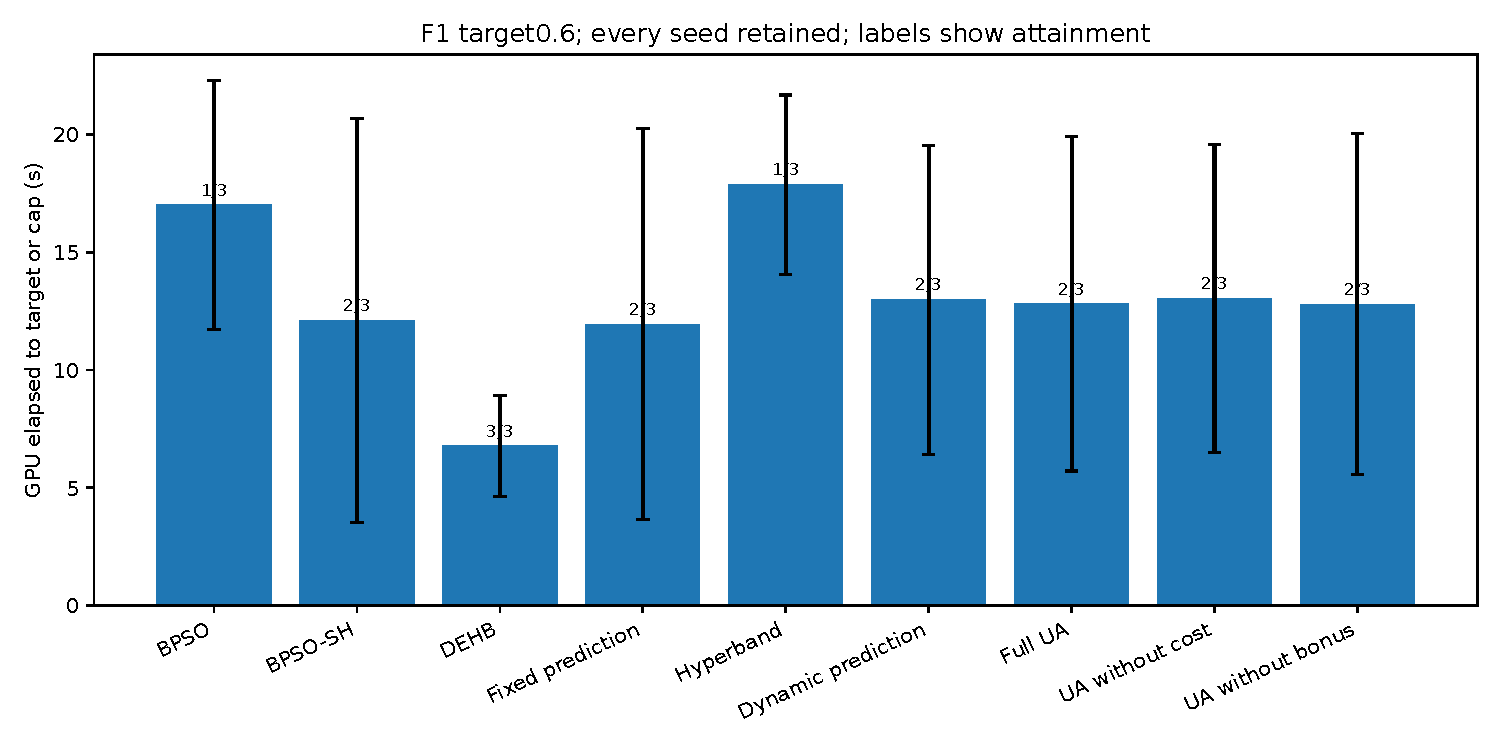
\includegraphics[width=\columnwidth]{target_cost_86ae7932.pdf}
\caption{Actual target-or-cap GPU consumption, including misses. Error bars show search-seed SD; annotations give target attainment.}\end{figure}
\begin{figure}[!t]\centering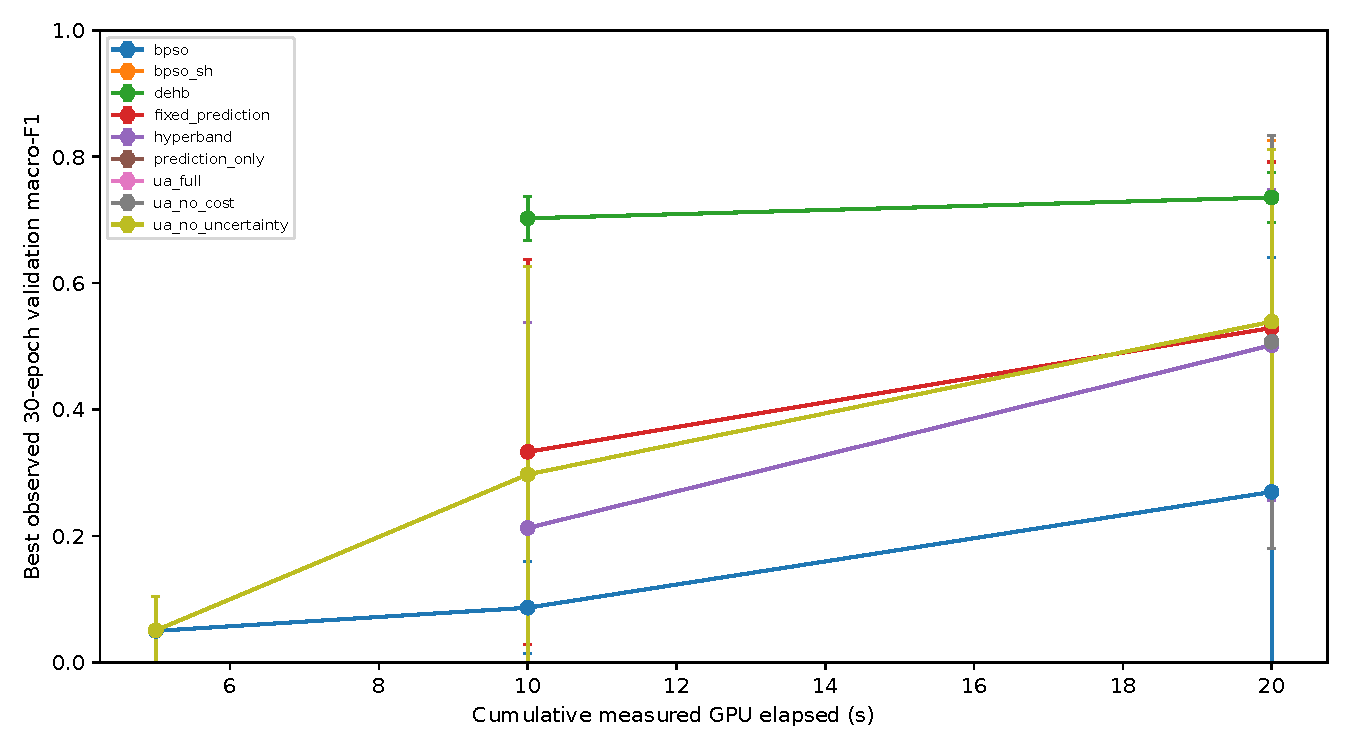
\includegraphics[width=\columnwidth]{gpu_anytime_014a9f0e.pdf}
\caption{Fixed-compute quality at 5/10/20 GPU seconds. Means/SD require all three seeds to have a terminal model; missing points are not replaced by zero. Raw seed traces are also retained.}\end{figure}
With a fixed 20-second compute allocation, mean validation macro-F1 was 0.5391 for full UA, 0.2696 for BPSO, 0.5030 for SH and 0.7356 for DEHB. The full-method gap to DEHB was 0.1965, exceeding the 0.02 preservation margin. Removing the uncertainty bonus changed no terminal winner scores. Removing cost reduced mean F1 by 0.0320, but cost-aware UA still did not beat SH on target-time cost. Fixed-quota prediction used 11.940 target-or-cap GPU seconds and F1~0.5291; dynamic prediction used 12.978 and 0.5071. The more complex allocation is not independently supported as an improvement.

\section{Total cost, final models and limitations}
Charging the historical archive gives 416.622 GPU seconds for one full-UA quality search versus 17.008 for BPSO: no net single-search saving remains. The fit/calibration subset alone cost 308.386 historical GPU seconds. Smaller-log CPU refits reduced that attributable subset but increased held-out point-prediction error; they were not substituted into the frozen benchmark. Historical reuse is not free computation. Online calibration was not claimed from a few adaptively selected terminal observations.

All methods' fixed-compute architecture choices were frozen before final testing, using dedicated seed 1601 and 30 epochs. The previously examined historical test is not blind independent data. BPSO test macro-F1 was 0.2733, with normal FPR 0.8038. BPSO-SH test macro-F1 was 0.5759, with normal FPR 0.6180; for Full UA, these values were 0.3100 and 0.9442, respectively. DEHB test macro-F1 was 0.6859, with normal FPR 0.7549. We retain precision, attack recalls, confusion matrices, parameters and measured inference latency. Generalization is limited by one final training seed and shared historical rows. The existing conventional MLP/CNN/GRU/reference results provide context.

At the preceding study stage, the regression suite passed 105 CPU tests and 50 targeted CUDA tests. We re-scored saved validation/test predictions and checked epoch ledgers.

DEHB is the strongest baseline. SH offers a simpler BPSO alternative and lower target-time cost than full UA. The runtime optimizations were verified. Novelty and superior uncertainty-aware allocation are \mbox{not established.} The~initial pilot (Section~\ref{sec:amf-measured}) and the archive-free online extension (Section~\ref{sec:amf-online}) are reported separately. More search/final \mbox{seeds, full-training} studies, independently validated calibration and independent captures are still needed.

\section{Archive-free online extension}
\label{sec:amf-online}
The archive-dependent result motivated a fresh experiment with separate bounds. Its implementation begins as ordinary BPSO--SH, with the same proposals, quotas and tie handling. It captures architecture, learning-curve prefix and measured incremental-cost features at epochs 3 and 10, attaching a terminal label only after actual epoch 30 training. No offline bundle, historical target, cross-method checkpoint or separately trained GPU archive enters this variant. Candidate maturation is charged to ordinary search work.

A fixed architecture hash assigns fit/calibration/check roles with expected proportions 50/20/30\%. CPU random forests use 24 trees of maximum depth 4. All current query architectures are excluded from fitting and calibration, and check forecasts are frozen before their terminal labels arrive. At least six fit, four calibration and four prequential check architectures per rung are required. The point gate requires MAE$\leq0.08$. MAE must be at least 10\% lower than that of current-F1 prediction. The absolute MAE improvement over that baseline must also be at least 0.005. The gate also requires Spearman$\geq0.3$. For uncertainty modes, empirical coverage must be at least 0.75 for nominal 80\% intervals, with mean width at most 0.3. Current intervals must also meet the width limit. These are conservative engineering checks, not a proof of calibration under adaptive sampling.

The interval uses a separate calibration quantile of absolute residual divided by forest dispersion (floor 0.02). When useful, ranking follows the earlier priority equation. It uses generic frozen values $\beta=0.1$ and $\lambda=0.05$, with median-normalized measured remaining cost. Prediction-only sets both coefficients to zero; uncertainty-only sets $\lambda=0$. If a gate fails, ordinary SH ranking remains in use. Swarm bests update only from actual terminal observations. We retain fixed SH quotas to isolate ranking, without claiming a new BPSO equation or algorithmic novelty.

\section{Fresh end-to-end comparison}
The 42 new runs use seeds 601--603 and seven methods. They include target 0.6 and fixed 20-GPU-second phases. Dataset rows, eight labels, preprocessing, architecture space, FP32 execution and 3/10/30 fidelities match the preceding 20-second experiment. A 50-second wall safety cap also applies. Methods run serially in a seeded permutation, without importing earlier checkpoints. Misses remain censored. Strict-horizon quality excludes terminal evaluations beyond the cap, while actual resource consumption includes epoch-boundary overruns. Timing follows the existing synchronized elapsed convention.

\begin{table}[!t]\centering\caption{Fresh target 0.6 runs, means across three search seeds. GPU seconds are measured; archive cost is charged to a standalone search. All misses are retained. Hits count actual terminal targets before the strict horizon.}\label{tab:online-quality}
\resizebox{\columnwidth}{!}{
\begin{tabular}{lrrrrr}\toprule
Method & Online GPU & Archive & Total GPU & F1 & Hits\\\midrule
BPSO & 16.824 & 0.00 & 16.824 & 0.3054 & 1/3\\
BPSO + SH & 12.004 & 0.00 & 12.004 & 0.4971 & 2/3\\
DEHB & 6.778 & 0.00 & 6.778 & 0.7026 & 3/3\\
Offline UA & 12.631 & 403.82 & 416.450 & 0.5391 & 2/3\\
Online prediction & 11.919 & 0.00 & 11.919 & 0.4971 & 2/3\\
Online + uncertainty & 11.950 & 0.00 & 11.950 & 0.4971 & 2/3\\
Archive-free full & 11.947 & 0.00 & 11.947 & 0.4971 & 2/3\\
\bottomrule\end{tabular}

}\end{table}

Archive-free full consumed 11.947 GPU seconds versus 16.824 for BPSO, a 28.99\% total reduction, with 2/3 versus 1/3 target attainment. Terminal validation macro-F1 means were 0.4971 and 0.3054, respectively. SH used 12.004 seconds. Its winner scores matched those of the archive-free variants. The small 0.47\% timing difference does not establish an advantage over SH. DEHB used 6.778 seconds and reached 3/3 targets. Removing the archive lowers standalone total cost relative to offline UA (416.450 seconds), but the online component itself must earn its cost.

Across the 18 matched online trials, predictive promotion activated 0 times and CPU fitting ran 0 times. Thus the new modes effectively executed SH in this short-horizon study. Their ablations do not establish any benefit from uncertainty or cost ranking. External archive cost is zero. This does not demonstrate an online-learning advantage. CPU preparation ranged 0.0017--0.0078 seconds per run and is included in search wall time.

With a fixed 20-second compute allocation, archive-free full preserved SH scores but trailed offline UA by 0.0361 and DEHB by 0.2325 absolute macro-F1. Both exceed the 0.02 engineering preservation margin; competitive quality against the strongest baseline was not maintained.

\begin{table}[!t]\centering\caption{Fresh fixed 20-GPU-second comparison. F1 is the best genuinely evaluated 30-epoch validation macro-F1, mean (sample SD). Epoch counts and actual GPU elapsed time include charged incremental work.}\label{tab:online-compute}
\resizebox{\columnwidth}{!}{
\begin{tabular}{lrrr}\toprule
Method & Terminal F1 (SD) & Epochs & GPU s\\\midrule
BPSO & 0.2696 (0.3715) & 178.7 & 20.040\\
BPSO + SH & 0.5030 (0.3231) & 138.3 & 20.088\\
DEHB & 0.7356 (0.0402) & 195.0 & 20.044\\
Offline UA & 0.5391 (0.2719) & 205.0 & 20.201\\
Online prediction & 0.5030 (0.3231) & 137.3 & 20.086\\
Online + uncertainty & 0.5030 (0.3231) & 137.3 & 20.089\\
Archive-free full & 0.5030 (0.3231) & 137.7 & 20.080\\
\bottomrule\end{tabular}

}\end{table}
\begin{figure}[!t]\centering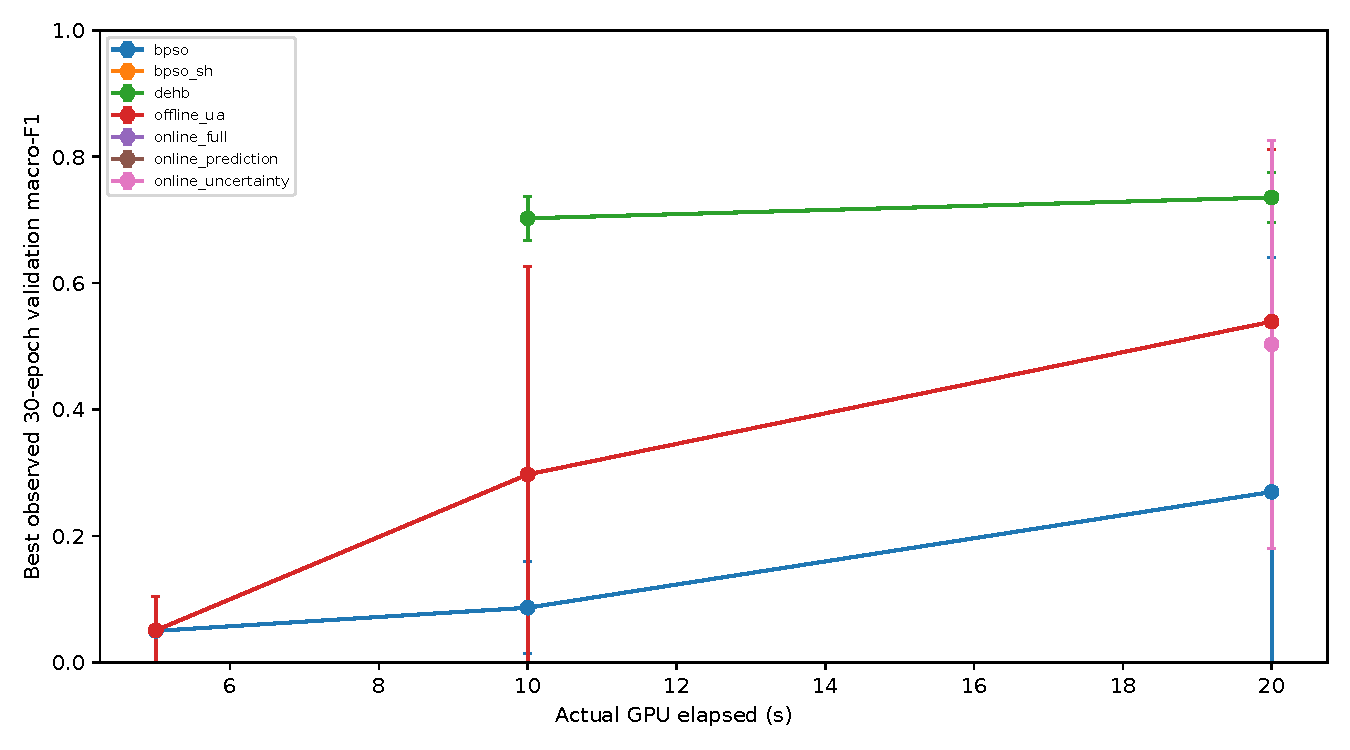
\includegraphics[width=\columnwidth]{anytime_d49e7dc1.pdf}
\caption{Fresh fixed-compute anytime quality. Error bars show search-seed SD; points require all three terminal scores. Equal compute consumption is not evidence of cost saving.}\end{figure}

The full archive is charged once for a reusable multi-search campaign in the accompanying CSV, rather than once per seed. Offline CPU development preparation is not fully isolated. The recorded archive wall time of 420.722 seconds is therefore only a lower bound for full offline wall preparation. We record online CPU fitting/inference and scheduler costs separately. All saved validation predictions were independently re-scored, and epoch/GPU ledgers and architecture-disjoint feature/predictor identities were verified. The expanded suite passed 110 CPU and 55 targeted CUDA-configured tests.

The separate seed 601 diagnostic used 120.061 GPU seconds and 128.449 wall seconds. It matured 16 distinct terminal architectures, performed 1 CPU fit and applied prediction at 0 promotion decisions. Preparation consumed 0.0475 CPU wall seconds. Prediction was blocked 32 times by too few fit or calibration architectures and once by too few out-of-time check architectures. This is a cold-start diagnostic, not a matched performance comparison.

No new final detector test was executed in this extension. The preceding historical test results are retained. The evidence supports removing an uneconomic archive and using SH fallback; it does not support superior online uncertainty-aware allocation. DEHB remains the strongest baseline, with SH the simpler BPSO alternative. Stronger conclusions about online prediction would require more seeds, a longer matched compute horizon, useful online calibration and independent data.
